\chapter{Postojeće metode detekcije objekata}


\section{R-CNN modeli}
\subsection{R-CNN} 
R-CNN ili "Region-Based Convolutional Neural Network" smatra se jednim od prvih većih
uspjeha u području detekcije objekata pomoću konvolucijskih neuronskih mreža.\citep{bworld}\newline
Ovaj model sastavljen je od 3 modula: 
\begin{description}
    \item [Prijedlog regija:]generiranje regija, tj. okvira oko mogućih objekata
    \item [Ekstraktor značajki:]konvolucijska neuronska mreža koja ekstrahira značajke iz svake predložene regije
    \item [Klasifikator:]klasificira značajke u neki od poznatih razreda
\end{description}


\begin{figure}[b]
    \centering
    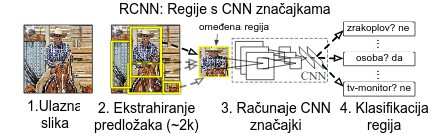
\includegraphics[width=10cm]{img/R-CNN.png}
    \caption{Koncept R-CNN modela. Slika preuzeta iz \citep{DBLP:journals/corr/GirshickDDM13}}.
    \label{fig:Koncept R-CNN modela}
\end{figure}

Model iz ulazne slike generira metodom selektivnog pretraživanja \engl{Selective search} regije koje bi mogle biti neki objekt
i šalje ih konvolucijskoj neuronskoj mreži da ekstrahira značajke. Za ovaj postupak uzeta je mreža "AlexNet deep CNN", koja 
šalje vektor značajki klasifikatoru.
Ovaj je postupak jednostavan i fleksibilan, ali je veoma spor. Razlog tomu je što se za svaku regiju (može ih biti i do 2000)
ponavlja gore navedeni postupak.\citep{DBLP:journals/corr/GirshickDDM13} \newline Slika \ref{fig:Koncept R-CNN modela} prikazuje ovaj postupak.
    


\subsection{Brzi R-CNN}
R-CNN, iako je bio veliki uspjeh, imao je svojih nedostataka.
Tako su u radu \cite{DBLP:journals/corr/Girshick15} navedeni neki nedostaci R-CNN-a : 
\begin{description}
    \item [Velike vremenske i prostorne složenosti:]treniranje na velikom broju regija
    \item [Detekcija objekata je spora:]detektiranje objekata je složeno zbog broja regija
\end{description}
Kao nadogradnju na R-CNN bio je predložen SPPnet \engl{Spatial Pyramid Pooling network}, koji smanjuje 
računanje generirajući mapu značajki za cijelu sliku.\newline Pomoću ove mape model može klasificirati svaki prijedlog objekta
koristeći vektor značajki ekstrahiran iz same mape.
Ovaj model bio je značajno brži od R-CNN-a (između 10 i 100 puta za vrijeme testiranja). Ovaj model je međutim morao spremati značajke u memoriju.\newline

Rješenje ovih problema je Brzi R-CNN sa sljedećim značajkama i prednostima:
\begin{enumerate}
    \item Veći mAP 
    \item Treniranje se odvija u jednom prolasku kroz mrežu koristeći MTL \engl{Multi task loss}
    \item Treniranje ažurira sve slojeve mreže
    \item Nema spremanja značajki u memoriju
\end{enumerate}

\begin{figure}[htb]
    \centering
    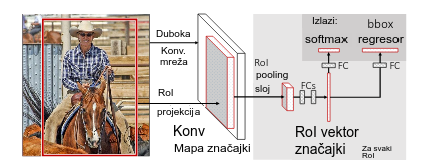
\includegraphics[width=10cm]{img/Fast-RCNN.png}
    \caption{Koncept Brzog R-CNN modela. Slika preuzeta iz \citep{DBLP:journals/corr/Girshick15}}
    \label{fig:Koncept Brzog R-CNN modela}
\end{figure}

Vjerojatno glavna značajka ovoga modela je regija interesa \engl{Region of interest}, koja ubrzava
detekciju samih objekata na ulaznoj slici. 
Značajke koje generira ovaj sloj šalju se dalje u potpuno povezane slojeve \engl{Fully connected layer} koji 
se na kraju račvaju u dva izlaza. Jedan izlaz daje vjerojatnost pojave pojedinog objekta u regiji, dok 
drugi kao rezultat daje dimenzije i koordinate okvira koji obavija sam objekt. Na slici \ref{fig:Koncept Brzog R-CNN modela} može se
vidjeti pojednostavljeni prikaz rada ovog modela. \cite{DBLP:journals/corr/Girshick15}


\subsection{Brži R-CNN}
Uspjeh prethodnih modela potaknuo je Girshicka i njegov tim da dalje razvijaju brže i preciznije modele.
Tako su razvili Brži R-CNN. Ovaj se model sastoji od dva modula.\newline
Prvi modul konvolucijska je neuronska mreža koja na temelju ulazne slike generira predložene regije za pojedine objekte, kao i vrijednost koja određuje pripada li ta regija
nekom razredu iz skupa razreda ili pozadini.

\begin{figure}[htb]
    \centering
    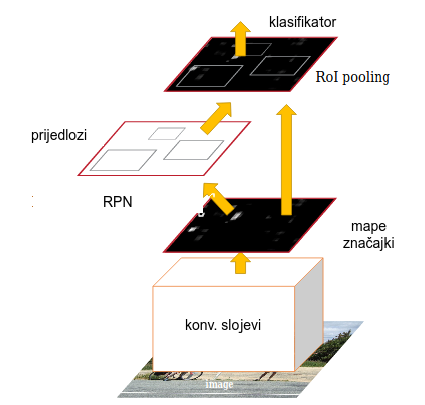
\includegraphics[width=10cm]{img/Faster-RCNN.png}
    \caption{Koncept Bržeg R-CNN modela. Slika preuzeta iz \citep{DBLP:journals/corr/RenHG015}}
    \label{fig:Koncept Bržeg R-CNN modela}
\end{figure}

Taj modul naziva se RPN \engl{Region Proposal Network}. Važnost ovog modula je što on predlaže drugom modulu gdje da pretražuje. Vrijednost koja označava pripadnost razredu ili pozadini 
omogućuje drugom modulu da brže klasificira i odredi poziciju objekta. 
Drugi modul zapravo je Brzi R-CNN. On iz predloženih regija ekstrahira značajke i na temelju njih daje kao izlaz oznaku razreda kojemu objekt pripada kao i dimenzije i poziciju okvira koji
omeđuje objekt.\newline
Značajke ovakve arhitekture su znatno smanjena količina generiranih regija i ubrzanje u samoj detekciji. Slika \ref{fig:Koncept Bržeg R-CNN modela} grafički prikazuje
ova dva modula \citep{DBLP:journals/corr/RenHG015}


\section{YOLO modeli}
RCNN modeli imaju svojih prednosti i mana. Kroz godine razvijanja modeli su značajno napredovali po pitanju preciznosti. 
U današnje je vrijeme međutim sve veća potreba za brzinom 
pojedinih modela pa RCNN modeli nisu najpraktičnija skupina modela za zadovoljavanje ovih potreba.\newline
YOLO \engl{You Only Look Once} modeli takva su vrsta modela. Nisu nužno precizniji od RCNN modela, ali su neusporedivo
brži i najčešće se koriste za detekciju u stvarnome vremenu \engl{Real-time object detection}. 


\subsection{YOLO}
U radu \citep{DBLP:journals/corr/RedmonDGF15} Joseph Redmon prvi je opisao ovu vrstu modela.\newline
U razvoju ovog modela sudjelovao je i sam Ross Girshick. 
Razlog zašto je ovakav model brži i bolji za uporabu u detektiranju objekata u stvarnome vremenu je korištenje konvolucijske neuronske
mreže koja u isto vrijeme pretpostavlja višestruke regije i razrede za iste. Glavna prednost YOLO modela je veoma velika brzina. Objekte na videozapisu može detektirati sa samo 25 milisekundi kašnjenja.\newline
Model radi na sljedeći način \citep{DBLP:journals/corr/RedmonDGF15}:\newline
\begin{enumerate}
    \item Ulaznu sliku dijeli na SxS kvadratnu mrežu, a S je proizvoljno odabran prirodni broj i predstavlja broj kvadrata u retku/stupcu mreže
    \item Ako se sredina objekta nađe unutar jednog kvadrata mreže, taj kvadrat je zadužen za detektiranje tog objekta
    \item Svaki kvadrat pretpostavlja
     \begin{itemize}
         \item  B okvira oko objekta, a B je proizvoljan prirodni broj okvira čija se težišnica nalazi unutar kvadrata.
        Svaki od B okvira sadrži strukturu podataka u kojoj su zapisani podaci o x i y koordinatama centra okvira u odnosu na rubove kvadrata. Isto tako su zapisani podaci o širini i 
          visini okvira u odnosu na cijelu sliku i vrijednost IoU između generiranog okvira i okvira temeljne istine za taj objekt
         \item  C vjerojatnosti pojave razreda iz skupa razreda, a C je broj razreda u skupu. Ove se vjerojatnosti računaju 
         samo ako je središte nekog objekta unutar kvadrata
    \end{itemize}
    \item Svaki okvir koji ima IoU manji od proizvoljne granice (na primjer 0.25 ili 0.5) se odbacuje
    \item Za preostale okvire se računa postotak koji označava sigurnost modela da se unutar okvira nalazi objekt iz razrednog skupa (na primjer "čovjek").
    Računa se kao umnožak IoU i vjerojatnosti pojave određenog razreda unutar kvadrata koji je zadužen za detekciju tog objekta.
\end{enumerate}
Slika ~\ref{fig:Rad YOLO modela} prikazuje gore navedeni postupak.
Kako bi se izbjeglo računanje rezultata u slučaju 
da je više kvadrata detektiralo isti objekt koristi se non-max potiskivanje. Non-max potiskivanje postupak je u kojem se uklanjaju višestruka pojavljivanja pretpostavljenog okvira za isti objekt.
\begin{figure}[htb]
    \centering
    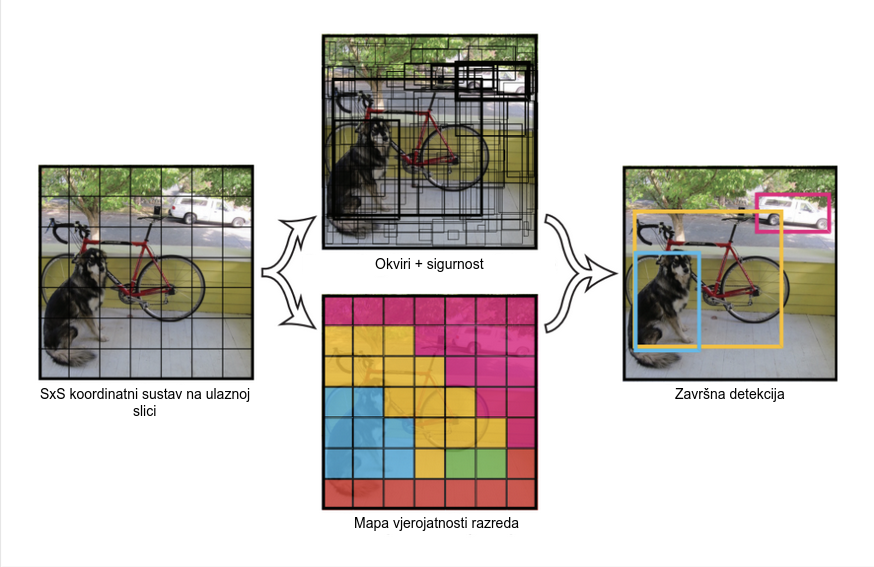
\includegraphics[width=12cm]{img/YOLO-process.png}
    \caption{Rad YOLO modela. Najprije je potrebno podijeliti sliku na SxS kvadratnu mrežu. Na ovoj slici S je 7 što znači 49 kvadrata.
    Zatim svaki od tih 49 kvadrata generira pretpostavljene okvire. U ovom slučaju generiraju se 2 okvira oko svakog kvadrata, što je prikazano na gornjoj sličici u sredini.
    Radi preglednosti su uklonjeni kvadrati. Na donjoj slici u sredini su vjerojatnosti pojave razreda grupirane po bojama. Izbacuju se 
    okviri s neodgovarajućom vrijednosti IoU. Zatim se množe vrijednost IoU iz preostalih okvira i vjerojatnost pojave razreda iz kvadrata oko kojih ti okviri jesu
    kako bi se dobili konačni okviri prikazani na posljednoj sličici. 
     Slika preuzeta iz \citep{DBLP:journals/corr/RedmonDGF15}}
    \label{fig:Rad YOLO modela} 
\end{figure}

Ograničenja su vidljiva prilikom detekcije manjih objekata u grupi, jer prilikom pretpostavljanja okvira  i određivanja 
razreda svaki kvadrat na kvadratnoj mreži može imati zapisane informacije o samo dva okvira i jednom razredu. 
YOLO, za razliku od RCNN-a, u obzir uzima cijelu sliku prilikom generiranja pretpostavki. Time smanjuje
stopu pogrešaka, jer ne obrađuje pozadine koje ne predstavljaju niti jedan razred. Ovaj model neće podbaciti kada se na ulazu nađe novi, dosad neviđeni 
objekt, jer ima veliku sposobnost generalizacije.\citep{DBLP:journals/corr/RedmonDGF15}   

Jedna od glavnih značajki YOLO modela jest povezanost više zasebnih komponenti u jednu neuronsku mrežu. 
Simultano pretpostavljanje okvira oko objekata i razreda čini ovaj model sofisticiranijim u odnosu na druge modele detekcije objekata. 


\subsection{YOLOv2}
Nadogradnja prethodne inačice modela, YOLOv2, uvodi nove značajke koje joj omogućuju još kvalitetniju detekciju objekata.\newline
Neki od novih dodataka su:
\begin{description}
    \item [Grupna normalizacija \engl{Batch normalization}:]podigla je mAP za 2\%
    \item [Klasifikator visoke rezolucije:]omogućen je unos slika visoke rezolucije, što rezultira povećanjem mAP-a od 4\%
    \item [Usidreni okviri \engl{Anchor Boxes}:]omogućuju lakše treniranje mreže
\end{description}

Zanimljivost ovog modela je implementacija nasumične promjene rezolucije ulazne slike svakih 10 grupa.
Autori modela su kao najmanju dimenziju odabrali 320x320, a 
kao najveću 608x608. Sve dimenzije između višekratnici su broja 32. \newline
Ovakav način treniranja omogućuje modelu prilagođavanje na različite rezolucije 
slika prilikom testiranja. \newline
Također, ovaj model je paralelno bio treniran na dva skupa podataka, COCO i ImageNet te može 
detektirati 9000 vrsta objekata u stvarnom vremenu. \citep{DBLP:journals/corr/RedmonF16}


\section{SSD}
SSD ili "Single Shot Detector" nastoji dodatno smanjiti kašnjenja i povećati preciznost prilikom detektiranja. 
Ovaj model koristi VGG16 kako bi ekstrahirao značajke iz ulazne slike. VGG16 predstavlja unaprijed treniranu konvolucijsku neuronsku mrežu koja služi za postavljanje 
parametara modela. 
Prvi sloj nakon VGG16 mreže služi za detekciju manjih objekata na slici i dimenzija je 38x38. Ova dimenzija predstavlja broj kvadrata na koje model dijeli sliku. 
Dimenzije naknadnih slojeva sve su manje (na primjer 8x8 i 4x4) i one služe detektiranju većih objekata na slici. 
Svaki kvadrat generira četiri pretpostavke za mogući objekt. Svaka pretpostavka sastoji se od okvira oko objekta 
i C + 1 vjerojatnosti pojavljivanja razreda unutar okvira, a C je broj razreda u razrednom skupu. Broj 1 predstavlja dodatan razred
kada ne postoji objekt unutar generiranog okvira i označen je brojem 0. Razred s najvećom vjerojatnošću uzima se kao pretpostavljeni razred 
za taj okvir. Na slici \ref{SSD okvir} prikazan je primjer generiranja okvira. Slika je preuzeta s \footnote{\url{https://cutt.ly/0yB2Odq}}


\begin{figure}[htb]
    \centering
    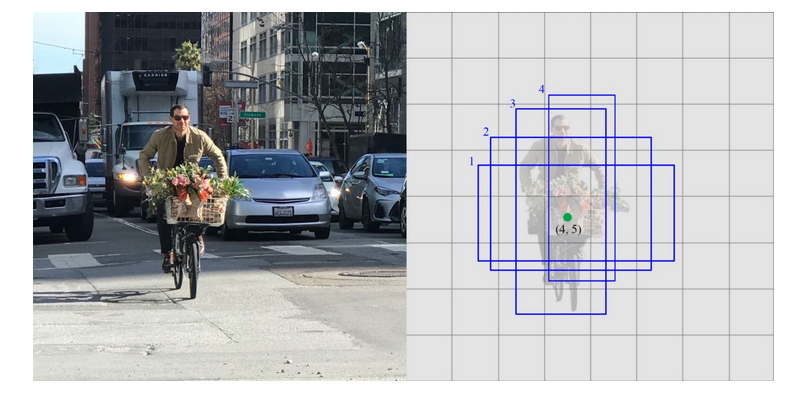
\includegraphics[width=10cm]{img/SSD-okviri.png}
    \caption{Lijevo na slici nalazi se originalna fotografija. Na desnoj slici vidi se generiranje četiri okvira oko pretpostavljenog objekta za kvadrat koji se 
    nalazi u 5 retku i 4 stupcu 8x8 mreže. Treba napomenuti da bi se ovaj postupak trebao izvodi u sloju koji je dimenzija 38x38, a da je zbog jednostavnijeg prikaza 
    taj sloj na slici prikazan kao kvadratna mreža dimenzija 8x8. U slojevima s manjim dimenzijama (8x8 ili 4x4) generira se šest pretpostavki}
    \label{SSD okvir}
\end{figure}

Uz generirane okvire, svaki kvadrat generira i unaprijed definirane okvire. Ovi okviri ručno su definirani kako bi mogli pokriti širok spektar objekata iz stvarnog svijeta.
U početnim slojevima s većim dimenzijama generiraju se četiri takva okvira, a u slojevima s manjim dimenzijama šest, isto kao što vrijedi za generiranje pretpostavki.
Generiranje ovih okvira smanjuje količinu računanja na početku treniranja.
Unaprijed definirani okviri koji imaju IoU s okvirom temeljne istine većim od 0.5 označuju se kao pozitivni, dok oni koji imaju IoU manji od te vrijednosti se označuju kao negativni.
Lokalizacijski gubitak računa se kao suma smooth L1 vrijednosti odstupanja pretpostavljenih okvira od okvira temeljne istine za sve pozitivno označene unaprijed definirane okvire nad svim razredima. 
Smooth L1 funkcija definira se kao 
\[
    smoothL1(x) = \left\{\begin{array}{lr}
        0.5x^2, & \text{ako } |x| <  1\\
        |x|- 0.5, & \text{inače } \\
        \end{array}\right\}
\]
i objašnjenje zašto se koristi nije u sklopu ovog rada. \citep{DBLP:journals/corr/LiuAESR15}
